\documentclass[12pt,a4paper,leqno]{report}

\usepackage[ansinew]{inputenc}
\usepackage[T1]{fontenc}
\usepackage[english]{babel}
\usepackage{amsthm}
\usepackage{amsfonts}         
\usepackage{amsmath}
\usepackage{amssymb}
\usepackage{enumitem}
\usepackage{fixltx2e}
\usepackage{tikz}
\usepackage{mathabx}
\usepackage[toc,page]{appendix}
\usetikzlibrary{calc}



\newcommand{\argmax}{\operatornamewithlimits{argmax}}
\newcommand{\R}{\mathbb{R}}
\newcommand{\C}{\mathbb{C}}
\newcommand{\Q}{\mathbb{Q}}
\newcommand{\N}{\mathbb{N}}
\newcommand{\No}{\mathbb{N}_0}
\newcommand{\Z}{\mathbb{Z}}
\newcommand{\diam}{\operatorname{diam}}
\newcommand{\ob}{\operatorname{ob}}

\newcommand\opn{\mathrel{\ooalign{$\subset$\cr
			\hidewidth\hbox{$\circ\mkern.5mu$}\cr}}}
\newcommand\cls{\mathrel{\ooalign{$\subset$\cr
			\hidewidth\hbox{$c\mkern.5mu$}\cr}}}
\newcommand*{\QEDA}{\hfill\ensuremath{\blacksquare}}%

\theoremstyle{plain}
\newtheorem{lause}[equation]{Theorem}
\newtheorem{lem}[equation]{Lemma}
\newtheorem{prop}[equation]{Proposition}
\newtheorem{kor}[equation]{Corollary}
\newtheorem{vaite}{V�ite}

\setcounter{secnumdepth}{3}
\newcounter{diagram}
\numberwithin{diagram}{subsection}
\newenvironment{diagram}
{\stepcounter{diagram}\par\smallskip\noindent\begin{minipage}{\linewidth}\centering}
	{\par Diagram~\thediagram\end{minipage}\par\smallskip}
\theoremstyle{definition}
\newtheorem{maar}[equation]{Definition}
\newtheorem{konj}[equation]{Conjecture}
\newtheorem{esim}[equation]{Example}

\theoremstyle{remark}
\newtheorem{huom}[equation]{Huomautus}

\pagestyle{plain}
\setcounter{page}{1}
\addtolength{\hoffset}{-1.15cm}
\addtolength{\textwidth}{2.3cm}
\addtolength{\voffset}{0.45cm}
\addtolength{\textheight}{-0.9cm}


\title{Cech (co)homology}
\author{Yury Elkin}
\date{}



\begin{document}

\maketitle

\tableofcontents

\chapter{Inroduction}\label{johd}



\chapter{Background}

In this chapter we will recall a few details about algebra, category theory and abstract simplicial complexes. We assume that the reader is familiar with basic concepts of homology and cohomology theory and constructions related to them.

\section{Direct sum and direct product}
In this section we will recall a few details about direct sums and direct products.
\begin{maar}
Let $\{A_i\}_{i \in J}$ be a family of groups. The direct product of these groups is the Cartesian product $\prod_{i \in J} A_i$ where addition is defined component-wise $(a+b)_i = a_i+_ib_i$
\end{maar}
\begin{maar}
Let $\{A_i\}_{i \in J}$ be a family of groups. The direct sum of these groups is the subgroup of direct product given by  $\bigoplus_{i \in J}A_i = \{x \in \prod_{i \in J} A_i \mid x_i \neq 0 \text{ for only finetely many } i \}. $
\end{maar}
For direct sums and direct products we have following universal properties:
\begin{lem}\label{Universalpropertyproduct}
Let $A = \prod_{i \in J} A_i$ be the direct sum and $D$ an arbitrary group. Then for every set of homomorphisms $\{f_i:D \rightarrow A_i\}_{i \in J}$ there exists a unique homomorphism $f:D \rightarrow A$ for which condition $pr_i \circ f = f_i $ holds for every $i \in J$.
\end{lem}
\begin{proof}
Proved in [\ref{algebra2}] theorem 3.7.
\end{proof}
\begin{lem}\label{Universalpropertysum}
	Let $A = \bigoplus_{i \in J}A_i$ be the direct sum and $D$ an arbitrary group. Then for every set of homomorphisms $\{f_i:A_i \rightarrow D\}_{i \in J}$ there exists a unique homomorphism $f:A \rightarrow D$ for which the condition $ f \circ j_i = f_i $ holds for every $i \in J$.
\end{lem}
\begin{proof}
Proved in [\ref{algebra2}] theorem 3.6.
\end{proof}
\section{Category theory}

In this thesis we will present theory in a categorical way, which will make the construction more general. First lets recall the definition of a category. 

\begin{maar}
A category C consist of the following ingredients: A class of objects $\ob(C)$, a class of morphisms $\hom(C)$ for which and for every objects $A$, $B$ in $\ob(C)$ there exists a subclass $Hom(A,B)$ and a rule of composition $Comp:Hom(A,B) \times Hom(B,D) \rightarrow Hom(A,D)$ for which following conditions hold:
\begin{enumerate}[label=(\arabic*),ref=(\arabic*)]
	
	
	\item Composition is associative. Let $f:A \rightarrow B$, $g: B \rightarrow D$ and $h: D \rightarrow E$ be morphisms between objects then $(f \circ g) \circ h = f \circ (g \circ h)$.
	
	\item For every object $A \in \ob(C)$ there exists identity morphism $1_A \in \hom(A,A)$ for which the following condition holds: Let $f:A \rightarrow B$ and $g: B \rightarrow A$ be arbitrary morphisms then $f \circ 1_A = f$ and $1_A \circ g = g$.
	
\end{enumerate}
\end{maar}
\begin{maar}
We say that a category $D$ is a subcategory of category $C$, if the following conditions are satisfied:
\begin{enumerate}[label=(\arabic*),ref=(\arabic*)]
	
	\item The collection of objects $\ob(D)$ is a subcollection of $\ob(C)$.
	\item The collection of morphisms $\hom(D)$ is a subcollection of $\hom(D)$.
	
\end{enumerate}
\end{maar}
\begin{maar}
Let $C$ be a category and $A, B$ its objects and let $f:A \rightarrow B$ be some morphism between them. We say that $f$ is an isomorphism, if there exists a morphism $g:B \rightarrow A$ for which the equations $g \circ f = id_A$ and $f \circ g = id_B$ hold. 
\end{maar}
It is easy to see that topological spaces with continuous functions and abelian groups with homomorphisms form a category. We denote those categories by TOP and AB. Next we will define the concept of a functor between categories.
\begin{maar}
Let $C$ and $C'$ be categories and let $F$ be a map between them. We say that $F$ is a functor between categories if the following conditions hold:

\begin{enumerate}[label=(\arabic*),ref=(\arabic*)]
	
	
	\item For every object $A \in \ob(C)$ there exists a unique object $F(A) \in C'$.
	
	\item Let $A$ and $B$ be objects in $\ob(C)$ and $f:A \rightarrow B$ a morphism between them. Then there exists a unique morphism $F(f):F(A) \rightarrow F(B)$.
	
	\item If $f$ and $g$ are morphisms in $\hom(C)$, then the following condition holds: $F(f) \circ F(g) = F(f \circ g)$.
	
	\item The identity element is mapped to the identity element. Let $A$ be an object in $\ob(C)$ and $1_A$ the identity morphism corresponding to it. Then $F(1_A)$ is the identity morphism of $F(A)$.
		

\end{enumerate}

\end{maar}
Homology and cohomology groups form a functor from TOP to AB. For details see Rotman [\ref{rotman}]. Now we will introduce a new concept called natural transformation.

\begin{maar}
Let $C$ and $D$ be categories and let $F:C \rightarrow D$ and $G:C \rightarrow D$ be functors. Then the following family of functors is a natural transformation: $$\{\phi_X: F(X) \rightarrow G(X)\}_{X \in C}$$ 
if the following conditions hold:
\begin{enumerate}[label=(\arabic*),ref=(\arabic*)]
	
	
	\item For every object $X \in C$ there exists a unique morphism $\phi_X: F(X) \rightarrow G(X) $
	
	\item For every morphism $f:X \rightarrow Y$ the following diagram commutes:
	
	$$ 	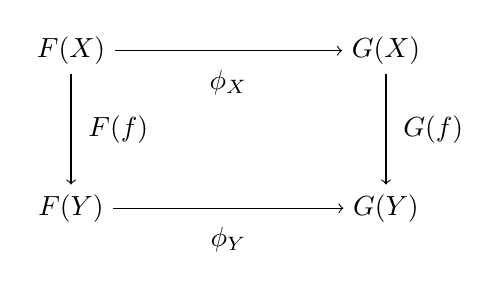
\begin{tikzpicture}
	
	
	
	\node (w) at (0,0) {\(F(X)\)};
	
	\node (x) at (0,-2) {\(F(Y)\)};
	
	\node (y) at (4,-2) {\(G(Y)\)};
	
	\node (z) at (4,0) {\(G(X)\)};
	
	\node (f) at (2,-2.4){\(\phi_Y\)};
	
	\node (g) at (2,-0.4){\(\phi_X\)};
	
	\node (s) at (0.6,-1) {\(F(f)\)};
	
	\node (s2) at (4.6,-1) {\(G(f)\)};	
	
	\draw[->] (z) -- (y);
	\draw[->] (w) -- (x);
	\draw[->] (x) -- (y);
	\draw[->] (w) -- (z);
	
	
	\end{tikzpicture}
	$$
	
	or in other words $\phi_Y \circ F(f) = G(f) \circ \phi_X $ holds.
	
\end{enumerate}
\end{maar}


Next we will define the concepts of limit and colimit for arbitrary categories, which will be later applied to direct and inverse systems.

\begin{maar}
	Let $C$ and $J$ be categories. We say that the category $C$ is indexed by the category $J$ if there exists a functor $F:J \rightarrow C$.	
\end{maar}	
We call the functor $F$ described above an indexing functor. It is easy to see that the functor induces a subcategory $F(J)$ of $C$. In the case where $F$ is indexing functor it is relatively easy to see that it is injective and thus we can equate $F(J)$ with $J$.
\begin{maar}
Let $C$ be a category indexed by $J$ and let $F:J \rightarrow C$ be the indexing functor. Let $N$ be a fixed object of the category $C$. We define the cone from $N$ to $F$ to be an indexed family of morphisms $$\Omega_N = \{\omega_X: N \rightarrow F(X)\}_{X \in J}$$ which satisfies the following property: If $f:X \rightarrow Y$ is a morphism in $C$ then the following diagram commutes


$$
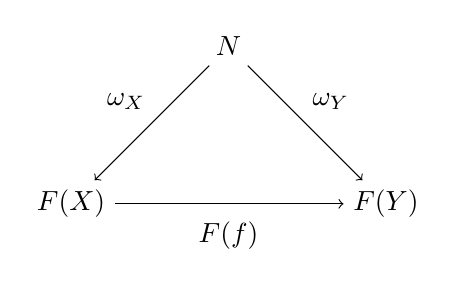
\begin{tikzpicture}

\node (w) at (2,0) {\(N\)};

\node (x2) at (0.7,-0.7) {\(\omega_X\)};

\node (x) at (0,-2) {\(F(X)\)};

\node (y2) at (3.3,-0.7) {\(\omega_Y\)};

\node (y) at (4,-2) {\(F(Y)\)};

\node (f) at (2,-2.4){\(F(f)\)};


\draw[->] (w) -- (y);
\draw[->] (w) -- (x);
\draw[->] (x) -- (y);


\end{tikzpicture}
$$
From now on we will denote the cone structure described above by $\bigtriangleup(F, N, \Omega_N)$. 
\end{maar}

\begin{maar}
Let $C$ be a category which is indexed by a category $J$ and let $F$ be the indexing functor. We say that the object $D \in \ob(C)$ is a limit of the functor $F$ if the following conditions are satisfied:
\begin{enumerate}[label=(\arabic*),ref=(\arabic*)]
\item There exists a family of morphisms $\Omega_D$ which induce the cone structure $\bigtriangleup(F, D, \Omega_D)$.
\item If $\bigtriangleup(F, N, \phi)$ is any other cone structure, then there exists a unique morphism $u:N \rightarrow D$ which makes the following diagram commute. 
\end{enumerate}
\end{maar}
$$
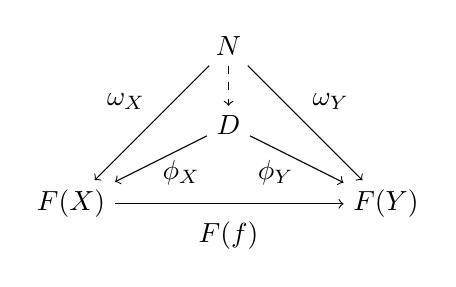
\begin{tikzpicture}

\node (w) at (2,0) {\(N\)};

\node (x2) at (0.7,-0.7) {\(\omega_X\)};

\node (x) at (0,-2) {\(F(X)\)};

\node (y2) at (3.3,-0.7) {\(\omega_Y\)};

\node (y) at (4,-2) {\(F(Y)\)};

\node (f) at (2,-2.4){\(F(f)\)};

\node (d) at (2,-1){\(D\)};

\node (phid) at (1.4,-1.6){\(\phi_X\)};
\node (phid2) at (2.6,-1.6){\(\phi_Y\)};


\draw[->] (w) -- (y);
\draw[->] (w) -- (x);
\draw[->] (x) -- (y);
\draw[dashed][->] (w) -- (d);
\draw[->] (d) -- (x);
\draw[->] (d) -- (y);


\end{tikzpicture}
$$
Next we will prove that if we have two limits $N$ and $D$ of a functor $F$ then there exists an isomorphism between those two objects. In other words $N$ and $D$ can be identified and the limit of the functor $F$ can be denoted simply as $\displaystyle {\lim_\rightarrow C}$ .

\begin{lause}
Let $F:J \rightarrow C$ be an indexing functor. Let $(N,\omega)$ and $(D, \phi)$ be limits of a functor $F$. Then there exists an isomorphism between them.
\end{lause}
\begin{proof}
Because $N$ and $D$ are both limits there exist morphisms $u: N \rightarrow D$ and $v: D \rightarrow N $ as above. Because of the symmetry it is enough to show that $v \circ u = id_N$. This follows directly from the equation $\omega_X \circ v \circ u  = \phi_X \circ u = \omega_X$. Because the diagram commutes for $id_N$ then by the uniqueness condition we see that $v \circ u = id_N$. 
\end{proof}
\subsection{Dual category}
To simplify definitions we will define the concept of a dual category. 
\begin{maar}
The dual of any concept in category theory can be obtained in the following way:
\begin{enumerate}[label=(\arabic*),ref=(\arabic*)]
	
	\item Interchange every occurrence of source with target
	\item Reorder every composition. That is, replace $a \circ b$ with $b \circ a$.
	
\end{enumerate}
%% Tarkistus suoritettu t�h�n asti
\end{maar}
Next we will give a few important examples of duality.
\begin{maar}
	Let $F:J \rightarrow C$ be the indexing functor. We define cocone to be the dual structure of the cone. 
\end{maar}
We will denote the cocone over an object $N$ as $\bigtriangledown(F,N,\Omega_N)$

\begin{maar}
	Let $C$ be a category which is indexed by a category $J$ and let $F$ be the indexing functor. We say that the object $D \in \ob(C)$ is a colimit of the functor $F$ if the following conditions are satisfied:
	\begin{enumerate}[label=(\arabic*),ref=(\arabic*)]
		\item There exists a family of morphisms $\Omega_D$ which induces a cocone structure $\bigtriangledown(F, D, \Omega_D)$.
		\item If $\bigtriangledown(F, N, \phi)$ is any other cocone structure, then there exists a unique morphism $u:D \rightarrow N$ which makes the following diagram commute. 
	\end{enumerate}
\end{maar}

$$
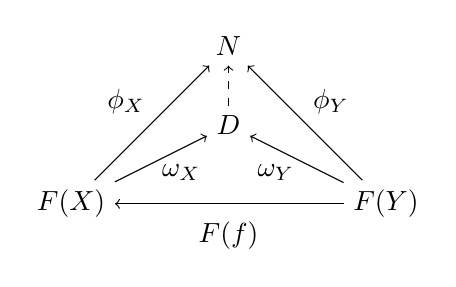
\begin{tikzpicture}

\node (w) at (2,0) {\(N\)};

\node (x2) at (0.7,-0.7) {\(\phi_X\)};

\node (x) at (0,-2) {\(F(X)\)};

\node (y2) at (3.3,-0.7) {\(\phi_Y\)};

\node (y) at (4,-2) {\(F(Y)\)};

\node (f) at (2,-2.4){\(F(f)\)};

\node (d) at (2,-1){\(D\)};

\node (phid) at (1.4,-1.6){\(\omega_X\)};
\node (phid2) at (2.6,-1.6){\(\omega_Y\)};


\draw[->] (y) -- (w);
\draw[->] (x) -- (w);
\draw[->] (y) -- (x);
\draw[dashed][->] (d) -- (w);
\draw[->] (x) -- (d);
\draw[->] (y) -- (d);


\end{tikzpicture}
$$

Like in the case of limits, colimits are unique. 

\begin{lause}
Let $F$ be an indexing functor and let $(N, \phi)$ and $(D, \omega)$ be colimits of $F$. Then there exists an isomorphism between the objects $N$ and $D$.
\end{lause}
\begin{proof}
Because $N$ and $D$ are both colimits there exist morphisms $u: N \rightarrow D$ and $v: D \rightarrow N $ as above. Because of the symmetry it is enough to show that $u \circ v = id_D$ holds. This follows from the equation $u \circ v \circ \omega_X = u \circ \phi_X = \omega_X$. The diagram commutes for $id_D$ and thus by the uniqueness condition we see that $u \circ v = id_D$. 
\end{proof}
\subsection{Direct and inverse systems}
In this section we will give a categorical definition of direct and inverse systems. It appears that those concepts are dual of each other. We will begin by defining a quasi-ordering relation:

\begin{maar}
Let $\lambda$ be a category and let $a \leq b$ be a relation in the object class $\ob(\lambda)$. We say that this relation is a quasi-ordering if the following conditions hold:
\begin{enumerate}[label=(\arabic*),ref=(\arabic*)]
	
	
	\item $a \leq a$ for all $a \in \ob(\lambda)$.
	\item If $a \leq b$ and $b \leq c$ then $a \leq c$ for all $a,b,c \in \ob(\lambda)$.
	
\end{enumerate}

\end{maar}
\begin{maar}
Let $\lambda$ be a category with a quasi-order relation. We say that the collection of morphisms correspond to the relation co-variantly, if the classes $\text{hom}(a,b) $ are of the following form:
$$\hom(a,b) = \left\{
\begin{array}{ll}
\{\lambda^a_b\}  & \mbox{if } b \leq a \\
\emptyset & \mbox{else.} 
\end{array}
\right.  $$ 
and the composition of two morphisms is defined to be $\lambda^b_a \circ \lambda^c_b = \lambda^c_a$ and the identity morphism to be $\lambda^a_a$.
\end{maar}
\begin{maar}
Respectively we say that the relation corresponds contra-variantly, if  

$$\hom(a,b) = \left\{
\begin{array}{ll}
\{\lambda^b_a\}  & \mbox{if } a \leq b \\
\emptyset & \mbox{else.} 
\end{array}
\right.  $$ 

the composition in which is defined to be $\lambda^c_b \circ \lambda^b_a = \lambda^c_a$ and the identity morphism to be $\lambda^a_a$.
\end{maar}
\begin{lem}
A quasi-ordered class of objects together with covariant or contra-variant class of morphisms forms a category.  
\end{lem}
\begin{proof}
We denote the object and morphism classes as defined above and prove that those collections satisfies the needed requirements to be called a category. For the covariant class, we have the following proof:
\begin{enumerate}[label=(\arabic*),ref=(\arabic*)]
	\item The associativity property: $(\lambda_c^d \circ \lambda^c_b) \circ \lambda^b_a = \lambda^d_a = \lambda_c^d \circ (\lambda^c_b \circ \lambda^b_a)$
	\item $\lambda^{a}_a \circ \lambda^b_a = \lambda^b_a $ and  $\lambda^{b}_a \circ \lambda^b_b = \lambda^b_a $ clearly holds

\end{enumerate}
The proof for the contra-variant is similar and we leave it to the reader to fill in the details.
\end{proof}
\begin{maar}
Let $\lambda$ be a quasi-ordered category. Let $C$ be a category and let $D:\lambda \rightarrow C$ be an indexing functor. If the morphism relation corresponds co-variantly to the relation we say that the functor $D$ is a direct system indexed by $\lambda$. In the case if the morphisms are contra-variant we denote the functor as $I$ and say that the functor is an inverse system indexed by $\lambda$.
\end{maar}


\begin{esim}
Let SET be the category of sets with order relation defined by $U \leq V \Leftrightarrow U \subset V$. Now for every $U,V$ we define $D_U^V: U \rightarrow V $ to be the inclusion from $U$ to $V$. Clearly this forms a direct system. 
\end{esim}

 Earlier we defined the concept of limit for general indexing functors. We can interpret direct and inverse system as indexing functors, taking $\lambda$ to be the indexing set. In general systems the limit may not exist. However, for our purpose it is enough to show that such limit can be found in the category of abelian groups.

\begin{lause}
Let $D:\lambda \rightarrow AB$ be a direct system of groups. For every $a \in \ob(\lambda)$ let $i_a: D(a) \rightarrow \bigoplus_{a \in \ob(\lambda)} D(a)$  be the inclusion and let $G$ be the subgroup of $D = \bigoplus_{a \in \lambda} D(a) $ which is generated by $\{i_ax_{a}-i_bD^b_ax_a\}$. Then the colimit of this system is the object $L = \bigoplus_{a \in \lambda} D(a) / G $.
\end{lause}
\begin{proof}
We denote $p$ to be the projection map: $p: \bigoplus_{a \in \ob(\lambda)} D(a) \rightarrow L$. Let $v$ be the family of morphisms $ \{v_a = p \circ i_a:D(a) \rightarrow L\}_{a \in \ob(\lambda)}$ which induces the cocone $\triangledown(D,L,v)$ and let $K$ be any other object with family of morphisms $\phi = \{\phi_a:D(a) \rightarrow K\}_{a \in \ob(\lambda)}$ which induces the cocone  $\triangledown(I,K, \phi)$. We have to prove that there exists a unique homomorphism $u:L \rightarrow K$ for which the condition $u \circ v_a = \phi_a $ holds for all $a \in \ob(\lambda)$. We will first show that such homomorphism exists \newline
Using lemma \ref{Universalpropertysum} we can find a unique homomorphism $u':\bigoplus_{a \in \lambda} D(a) \rightarrow K$ for which $u' \circ i_a = \phi_a$ holds. Now we see that for every generator of the subgroup G the following equations hold: $$u'(i_ax_{a}-i_bD^b_ax_a) = \phi_a(x_a) - \phi_bD_a^bx_a = \phi_a(x_a)-\phi_a(x_a) = 0.$$ Now we can define $u$ in such way that it maps every element $x + D$ to element $\phi'(x)$. Now we see that $$u \circ v_a = u \circ p \circ i_a = u' \circ i_a = \phi_a.$$
To prove that the homomorphism $u$ is unique we notice that if $x \in L$ , then $x = \sum_{a \in A \subset D} v_a(x_a) + G$.  Then the following equations hold  $$u(x) = u(\sum_{a \in A \subset D}v_a(x_a)) = \sum_{a \in A \subset D} u \circ v_a (x_a) = \sum_{a \in A \subset D} \phi_a(x_a)$$
Thus $u(x)$ is determined by the sum of the homomorphisms $\phi_a$. It follows that the map $u$ is unique.
\end{proof}
\begin{lause}
Let $I: \lambda \rightarrow AB$ be an inverse system of groups. Then the limit of this functor is the group $L = \{x \in \prod_{i \in \ob(\lambda)} I_i \mid x_a = I^b_ax_b $ for all $a \leq b\}$
\end{lause}
\begin{proof}
Let  $v$ be a family of homomorphisms $\{v_a = pr_a: L \rightarrow I(a)\}_{a \in \lambda}$ which together with the group $L$ induce the cone $\bigtriangleup(I,L,v)$. Let $K$ be any other group and let $\phi$ be a family of homomorphisms $\{\phi_a: K \rightarrow I(a)\}_{a \in \lambda}$ which induces the cone $\bigtriangleup(I,K,\phi)$ . \newline 
We construct a function $u: K \rightarrow L$ for which $v_a \circ u = \phi_a$ holds. Using lemma \ref{Universalpropertyproduct} we find a unique homomorphism $u':K \rightarrow \prod_{i \in J}I_i$ for which $pr_a \circ u' = \phi_a$ is satisfied. Let $u''$ be the homomorphism, where the image is restricted to subgroup $L$. We will show that the homomorphism is well-defined, specifically $u'$ maps every element inside the subgroup $L$. Assume that $b$ and $a$ are elements which satisfy the condition $a \leq b$. Then the following equation holds
 $$I^{b}_a \circ pr_b \circ u'= I^{b}_a \circ \phi_b = \phi_a = pr_a \circ u'.$$
  We can define $u$ to be $u''$. The uniqueness property of the homomorphism follows directly from the fact that $u'$ is unique. 
\end{proof}

\subsection{Morphisms between systems}\label{limitmorphism}
\subsubsection{Morphisms between inverse systems}

To be able to define morphisms between Cech homology groups we need the concept of a limit homomorphism. In this section we will define the limit morphism between systems and investigate properties of it. Concepts used in this chapter can be presented in a more general way. However, for our use it is enough to restrict ourselves to the direct and inverse system.

\begin{maar}
Let $C$ and $D$ be categories with order relation. A functor $\phi:C \rightarrow D$ is order preserving if for every pair $a \leq b$ in the category $C$, the condition $\phi(a) \leq \phi(b)$ is satisfied.
\end{maar}
 Let $I$ be an inverse system and $\phi: \lambda' \rightarrow \lambda$ an order preserving functor. Then the inverse system $(I \phi, \lambda' )$ consist of objects $\{I(\phi(a)) \mid a \in \ob(\lambda')\}$ and morphisms $\{I^{\phi(b)}_{\phi(a)}\mid a \leq b \}$.


\begin{maar}
Let $(I,\lambda)$ and $(I',\lambda')$ be inverse systems and $\phi:\lambda' \rightarrow \lambda$ an order and limit preserving functor. Let $ \{f_a:I(\phi(a)) \rightarrow I'(a) \mid a \in \lambda\}$ be a natural transformation between $I\phi$ and $I'$. Then we say that $\{f_a\}_{a \in \lambda}$ is an inverse system of morphisms corresponding to the functor $\phi$ from the system $I$ into the system $I'$.
\end{maar}

In the next theorem we will prove that it is possible to define the limit of morphisms between systems in a unique way. We recall that exists of limit implies that for every objects of category $I$ there exists unique functor $u_{I,a}:\lim I \rightarrow I(a)$.

\begin{lem}
Let  $(I,\lambda)$ and $(I',\lambda')$ be inverse systems for which limit exists. Let $\{f_a\}$ be inverse system of morphisms corresponding to that pair. Then there exists a unique morphism $\lim f:\lim I \rightarrow \lim I'$ for which the condition $\lim f \circ u_{I, \phi(a)} = u_{I',a} \circ f_a$ holds for every $a \in \lambda'$ .
\end{lem}
\begin{proof}
Consider the following diagram
\begin{diagram}\label{morphismbetweenlimits}
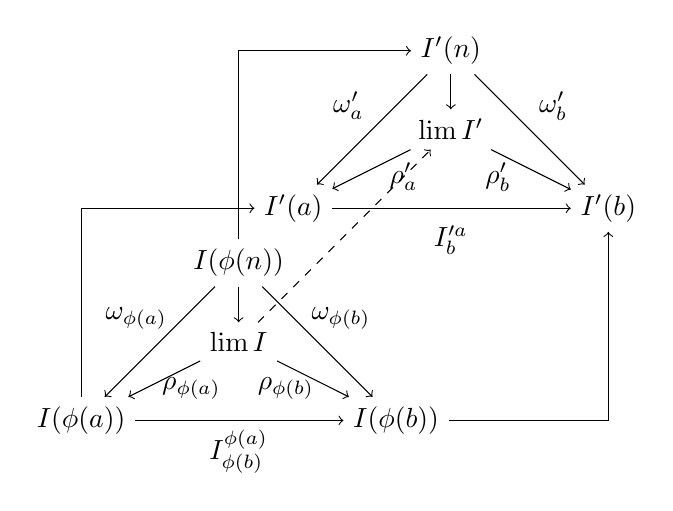
\begin{tikzpicture}

\node (w) at (2,0,0) {\(I(\phi(n))\)};

\node (x2) at (0.7,-0.7,0) {\(\omega_{\phi(a)}\)};

\node (x) at (0,-2,0) {\(I(\phi(a))\)};

\node (y2) at (3.3,-0.7,0) {\(\omega_{\phi(b)}\)};

\node (y) at (4,-2,0) {\(I(\phi(b))\)};

\node (f) at (2,-2.4,0){\(I^{\phi(a)}_{\phi(b)}\)};

\node (d) at (2,-1,0){\(\lim I\)};

\node (phid) at (1.4,-1.6,0){\(\rho_{\phi(a)}\)};
\node (phid2) at (2.6,-1.6,0){\(\rho_{\phi(b)}\)};

\node (w2) at (2,0,-7) {\(I'(n)\)};

\node (x22) at (0.7,-0.7,-7) {\(\omega'_a\)};

\node (x2) at (0,-2,-7) {\(I'(a)\)};

\node (y22) at (3.3,-0.7,-7) {\(\omega'_b\)};

\node (y2) at (4,-2,-7) {\(I'(b)\)};

\node (f2) at (2,-2.4,-7){\(I'^{a}_{b}\)};

\node (d2) at (2,-1,-7){\(\lim I'\)};

\node (phid2) at (1.4,-1.6,-7){\(\rho'_a\)};
\node (phid22) at (2.6,-1.6,-7){\(\rho'_b\)};

\draw[->] (w) -- (y);
\draw[->] (w) -- (x);
\draw[->] (x) -- (y);
\draw[->] (w) -- (d);
\draw[->] (d) -- (x);
\draw[->] (d) -- (y);

\draw[->] (w2) -- (y2);
\draw[->] (w2) -- (x2);
\draw[->] (x2) -- (y2);
\draw[->] (w2) -- (d2);
\draw[->] (d2) -- (x2);
\draw[->] (d2) -- (y2);

\draw[->] (w) |- (w2);
\draw[->] (x) |- (x2);
\draw[->] (y) -| (y2);


\draw[dashed][->](d) -- (d2);


\end{tikzpicture}
\end{diagram}

To prove that the limit morphism exists we form the following triangle out of the diagram described above:

$$
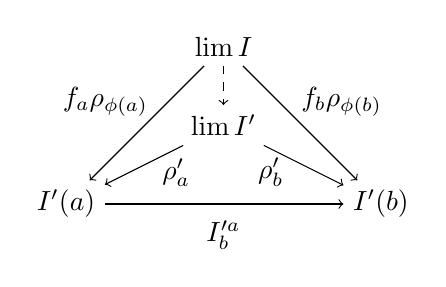
\begin{tikzpicture}

\node (w) at (2,0) {\(\lim I\)};

\node (x2) at (0.5,-0.7) {\(f_a \rho_{\phi(a)}\)};

\node (x) at (0,-2) {\(I'(a)\)};

\node (y2) at (3.5,-0.7) {\(f_b \rho_{\phi(b)}\)};

\node (y) at (4,-2) {\(I'(b)\)};

\node (f) at (2,-2.4){\(I'^{a}_{b}\)};

\node (d) at (2,-1){\(\lim I'\)};

\node (phid) at (1.4,-1.6){\(\rho'_a\)};
\node (phid2) at (2.6,-1.6){\(\rho'_b\)};


\draw[->] (w) -- (y);
\draw[->] (w) -- (x);
\draw[->] (x) -- (y);
\draw[dashed][->] (w) -- (d);
\draw[->] (d) -- (x);
\draw[->] (d) -- (y);


\end{tikzpicture}
$$
Then by definition of limit there exists a unique morphism $\lim f:\lim I \rightarrow \lim I'$ for which the diagram commutes. We will prove now that the universal property $\lim f \circ u_{I, \phi(a)} = u_{I',a} \circ f_a$ holds for this morphism. By diagram \ref{morphismbetweenlimits} and the fact that the family of functions $\{f_a\}$ is a natural transformation, in other words the condition $\omega'_a \circ f_n = f_a \circ \omega_{\phi(a)}$ holds, the following diagram commutes:
$$
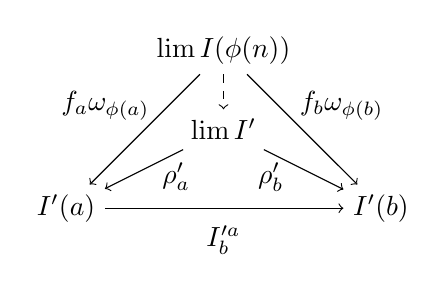
\begin{tikzpicture}

\node (w) at (2,0) {\(\lim I(\phi(n))\)};

\node (x2) at (0.5,-0.7) {\(f_a \omega_{\phi(a)}\)};

\node (x) at (0,-2) {\(I'(a)\)};

\node (y2) at (3.5,-0.7) {\(f_b \omega_{\phi(b)}\)};

\node (y) at (4,-2) {\(I'(b)\)};

\node (f) at (2,-2.4){\(I'^{a}_{b}\)};

\node (d) at (2,-1){\(\lim I'\)};

\node (phid) at (1.4,-1.6){\(\rho'_a\)};
\node (phid2) at (2.6,-1.6){\(\rho'_b\)};


\draw[->] (w) -- (y);
\draw[->] (w) -- (x);
\draw[->] (x) -- (y);
\draw[dashed][->] (w) -- (d);
\draw[->] (d) -- (x);
\draw[->] (d) -- (y);


\end{tikzpicture}
$$
Both maps $\lim f \circ u_{I, \phi(a)}$ and $u_{I',a} \circ f_a$ complete the diagram. Thus by uniqueness of the map corresponding to limit, we can conclude that the functions are same.

\end{proof}
For composition of two limits we have following result:

\begin{lem}\label{compositionlimitmorphism}
Let $(I, \lambda)$, $(I',\lambda')$ and $(I'',\lambda'')$ be inverse systems with limits and let $\phi:\lambda' \rightarrow \lambda$ and $\phi':\lambda'' \rightarrow \lambda'$ functors between systems. Let $ \{f_a:I(\phi(a)) \rightarrow I'(a) \mid a \in \phi'(\lambda'')\}$ and $ \{g_a:I'(\phi(a)) \rightarrow I''(a) \mid a \in \lambda''\}$ be families of morphisms corresponding to $\phi$ and $\phi'$. Let $\lim(f \circ g):I \rightarrow I''$ be the limit of the family $\{g_af_{\phi(a)}:I(\phi \phi'(a)) \rightarrow I''(a) \mid a \in \lambda''\}$.  Then $\lim(f \circ g) = \lim f \circ \lim g $ holds.
\end{lem}
\begin{proof}
To prove this we will use previous lemma and following commutative diagram:
	$$
	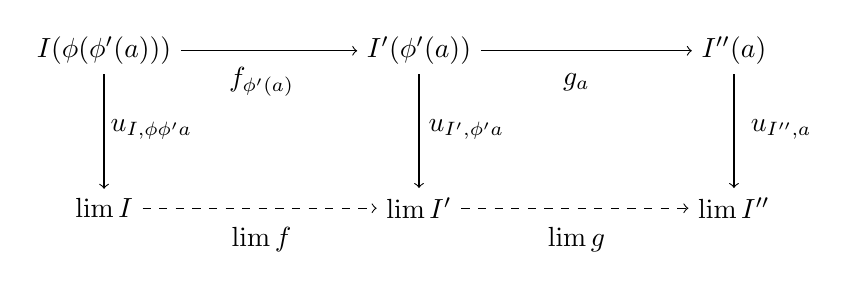
\begin{tikzpicture}
	
	
	
	\node (w) at (0,0) {\(I(\phi(\phi'(a)))\)};
	
	\node (x) at (0,-2) {\(\lim I\)};
	
	\node (y) at (4,-2) {\(\lim I'\)};
	
	\node (z) at (4,0) {\(I'(\phi'(a))\)};
	
	\node (p) at (8,0) {\(I''(a)\)};
	
	\node (p2) at (8,-2) {\(\lim I''\)};
	
	\node (f) at (2,-2.4){\(\lim f\)};\
	
	\node (f2) at (6,-2.4){\(\lim g\)};
	
	\node (g) at (2,-0.4){\(f_{\phi'(a)}\)};
	
	\node (g2) at (6,-0.4){\(g_{a}\)};
	
	\node (s) at (0.6,-1) {\(u_{I,\phi \phi'a}\)};
	
	\node (s2) at (4.6,-1) {\(u_{I', \phi'a}\)};	
	
	\node (s3) at (8.6,-1) {\(u_{I'', a}\)};	
	
	\draw[->] (z) -- (y);
	\draw[->] (w) -- (x);
	\draw[dashed][->] (x) -- (y);
	\draw[->] (w) -- (z);
	\draw[dashed][->] (y) -- (p2);
	\draw[->] (p) -- (p2);
	\draw[->] (z) -- (p);
	
	
	\end{tikzpicture}
	$$
	By definition of limit morphism the condition $\lim (f \circ g) \circ u_{I, \phi(\phi'(a))} = u_{I'',a} \circ (g_a \circ f_{\phi(a)})$ holds for the limit of the composition. By uniqueness of the limit homomorphism it is enough to show that the composition of two limit functors satisfies the condition. This follows from the following equations:
	$$\lim g \circ \lim f \circ u_{I, \phi(\phi'(a))} = \lim g  \circ u_{I', \phi'(a)} \circ f_{\phi'(a)} = u_{I'',a} \circ g_a \circ f_{\phi'(a)} $$
	

\end{proof}

Now we would like to define limit for the system of homomorphisms between inverse systems of groups.

\begin{lem}\label{limitmorphismgroup}
Let $(I, \lambda)$ and $(I',\lambda')$ be inverse systems of groups. Then $$f:\lim_{\rightarrow} I \rightarrow \lim_{\rightarrow}I' : f(x) = \prod_{a \in \lambda}f_a(proj_{\phi(a)}(x))$$
is a well defined homomorphism between the limit groups.
\end{lem}
\begin{proof}
We have to show that the image is in the subgroup $$L = \{x \in \prod_{i \in \lambda'} I'(i) \mid x_a = I^b_ax_b \text{ for all } a \leq b \}.$$ Let $b$ be some index, then: $I'^{b}_{a}x'_b = I'^{b}_{a}f_b(x_{\phi(b)}) = f_bI'^{\phi(b)}_{\phi(a)}(x_{\phi(b)}) = f_ax_{\phi(a)} = x'_a$ . In this equation we used the property which says that the morphisms define a natural transformation.
\end{proof}

\subsection{Finality properties of subsystems}
Final and cofinal functors can be defined in a more general way [\ref{categorytheory}]. However, because we are mainly interested in properties of systems, in this section we will investigate the properties of those specific functors only in that special case. In the case of general categories, cofinality includes a concept of connectedness defined in [\ref{categorytheory}] page 217. In our definition we will use a stronger version of that concept.

\begin{maar}
	Let $\lambda$ be a category with a quasi-order relation on its objects. We say that $\lambda$ is directed category, if for every two objects $a \in \lambda$ and $b \in \lambda$ we find object $c \in \lambda$ for which relations $a \leq b$ and $ a \leq c$ hold. 
\end{maar}
\begin{maar}
	Let $\lambda$ be a category with a quasi-order relation on its objects and $\lambda'$ its directed subcategory for which following condition holds: $$\text{For every }a \in \lambda \text{ there exists } b \in \lambda' \text{ for which } a \leq b.$$
	Then we say that $\lambda'$ is dense in $\lambda$. 
\end{maar}

\begin{maar}
Let $\lambda$ be a directed category with a quasi-order relation on its objects and let $\lambda'$ be its subcategory. Then we say that $\lambda'$ is a cofinal subcategory of $\lambda$, if $\lambda'$ is dense in $\lambda$.
\end{maar}
\begin{lem}\label{subcategorydirectness}
Let $\lambda$ be a directed category and $\lambda'$ its dense subcategory. Then $\lambda'$ is directed category. 
\end{lem}
\begin{proof}
Let $\alpha$ and $\beta$ be objects of $\lambda$. Then there exists $t \in \lambda$ for which $\alpha \leq \gamma$ and $\beta \leq \gamma$ hold. By density property there exists $\gamma' \in \lambda'$ for which condition $\gamma \leq \gamma'$ holds. Now claim follows directly from the equations $\alpha \leq \gamma \leq \gamma' $ and $\beta \leq \gamma \leq \gamma'$. 
\end{proof}

Now for the inverse system we have the following theorem:

\begin{lause}
Let $(I,\lambda)$ be an inverse system and let $(I',\lambda')$ be its subsystem generated by a cofinal subcategory $\lambda$. Assume that there exists a limit object for $I'$. Then the limit of the system $(I,\lambda)$ is $\lim I'$.

\end{lause}
\begin{proof}
Let $\lim I'$ be the limit of the inverse system $I'$. It is enough to show that $\lim I'$ is also the limit of $I$. We will first show that $\lim I'$ forms a cone in $I$ and then prove that for any other cone induced by an object $N$ in $I$ there exists a unique morphism $u:N \rightarrow \lim I'$. \newline
 Let $a$ be an arbitrary object of the indexing category $\lambda$. Then by the definition of cofinal subcategory there exists element $a' \in \lambda'$ for which $a \leq a'$ holds. Thus there exists a morphism $I^{a'}_a$. Because $\lim I'$ is the limit of the inverse system $I'$ it forms a cone $\bigtriangleup(I',\lim I',\rho)$, where $\rho$ is some collection of morphisms $\{\rho_{a}: \lim I' \rightarrow I'(a)\}_{a \in \ob(\lambda')}$. Using $\rho$ we form a new collection of morphisms $\rho'$ defined by $\{I^{a'}_a \circ \rho_{a'}\}_{a \in \ob(\lambda)} $. Because $I^{a'}_a \circ \rho_{a'}$ can vary on the choice of $a$, the composition may be not uniquely determined. However, if $a''$ is another object of $\lambda'$ for which the relation $a \leq a''$ holds, by lemma \ref{subcategorydirectness} there exists an object $t \in \lambda'$ for which the conditions $a \leq t$ and $a'' \leq t$ are satisfied. Because the following equations hold $$I^{a'}_a \circ \rho_{a'} = I^{a'}_a \circ I^{t}_{a'} \circ \rho_t = I^t_a \circ \rho_t = I_a^{a''} \circ I^{t}_{a''} \circ \rho_{t} = I^{a''}_a \circ \rho_{a''}$$ 
 we can conclude that $I^{a'}_a \circ \rho_{a'} = I^{a''}_a \circ \rho_{a''}$ and thus the family of homomorphisms is well-defined and $\lim(I')$ forms a cone $\bigtriangleup(I,\lim I', \rho' )$\newline
 Now if there exists another cone $\bigtriangleup(I,N,\omega)$ , we have to construct a morphism $u:N \rightarrow \lim I'$ and prove that it is unique. Let $a$ and $b$ be objects of $\lambda$, then there exists objects $a'$ and $b'$ in $\lambda'$ for which relations $a \leq a'$ and $b \leq b'$ hold. Restricting the collection $\omega$ to the morphisms indexed by $\lambda'$ we get the cone $\bigtriangleup(I',N,\omega')$ of $I'$. Because $\lim I'$ is the limit of the functor $I'$, there exists a unique homomorphism $u:N \rightarrow \lim I'$. It is left to prove that the following diagram commutes:
  $$
 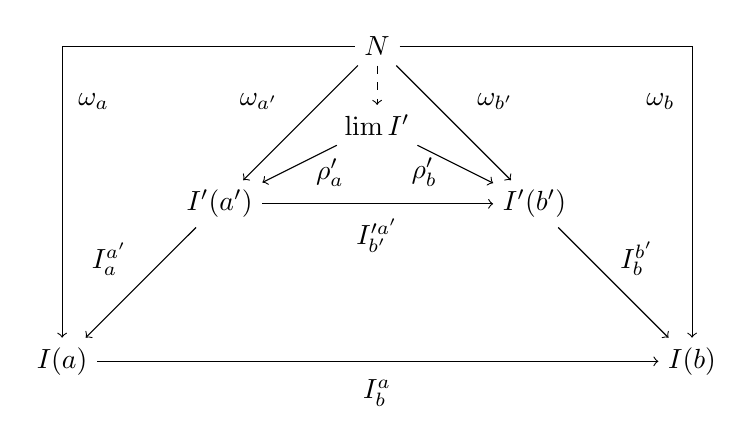
\begin{tikzpicture}
 
 \node (w) at (2,0) {\(N\)};
 
 \node (x2) at (0.5,-0.7) {\(\omega_{a'}\)};
 
  \node (x3) at (-1.6,-0.7) {\(\omega_{a}\)};
 
 \node (a2) at (-1.4,-2.7) {\(I^{a'}_{a} \)};
 
 \node (x) at (0,-2) {\(I'(a')\)};
 
 \node (y2) at (3.5,-0.7) {\(\omega_{b'}\)};
 
   \node (y3) at (5.6,-0.7) {\(\omega_{b}\)};
 
  \node (b2) at (5.3,-2.7) {\(I^{b'}_{b} \)};
 
 \node (y) at (4,-2) {\(I'(b')\)};
 
 \node (f) at (2,-2.4){\(I'^{a'}_{b'}\)};
 
  \node (f2) at (2,-4.4){\(I^{a}_{b}\)};
 
 \node (d) at (2,-1){\(\lim I'\)};
 
 \node (phid) at (1.4,-1.6){\(\rho'_a\)};
 \node (phid2) at (2.6,-1.6){\(\rho'_b\)};
 
 \node(a) at (-2,-4) {\(I(a)\)};
  \node(b) at (6,-4) {\(I(b)\)};
 
 \draw[->] (w) -- (y);
 \draw[->] (w) -- (x);
 \draw[->] (x) -- (y);
 \draw[dashed][->] (w) -- (d);
 \draw[->] (d) -- (x);
 \draw[->] (d) -- (y);
 \draw[->] (x) -- (a);
 \draw[->] (y) -- (b);
 \draw[->] (a) -- (b);
 \draw[->] (w) -| (a);
 \draw[->] (w) -| (b);
 
 
 
 \end{tikzpicture}
 $$
 Especially we have to prove that $I^{a'}_{a} \circ w_{a'} = w_a $ . This claim follows directly from the fact that $\bigtriangleup(I,N,\omega) $ is a cone. Thus the $u$ defined above is the map we were searching for.

\end{proof}


\section{Nerve of covering}
In this chapter we will give a definition of an abstract simplicial complex. 


\subsection{Abstract simplicial complex}
We assume that the reader knows already basic facts about simplicial complexex. If not we suggest to take a look at [\ref{rotman}]. 
\begin{maar}
	Let $S$ be some simplex and let $X$ be a collection of its faces. We define operator $\rhd:2^{X} \rightarrow X$ to denote a simplex which is obtained by the intersection of all simplexes for which the union of all the faces in the domain are contained. 
\end{maar}

\begin{maar}
Let $X$ be a set and let $\mathcal{A} = \{S_i\}_{i \in J}$ be some collection of finite subsets of the set $X$. We say that $\mathcal{A}$ forms an abstract simplicial complex over $X$, if a subset of any set $S_i$ in the collection $\mathcal{A}$ is in the collection.
\end{maar}
For an abstract simplicial complex we define the following geometric structure which will give us the interface of original simplicial complex. 
\begin{maar}
Let $X$ be a topological space and $\mathcal{S}(X)_\mathcal{A}$ abstract simplicial complex induced by $X$ and some covering $\mathcal{A}$ and let $J$ be its vertex set. Then the geometric realization of the abstract simplicial complex $\mathcal{S}(X)_\mathcal{A}$ is a subset of the set $[0,1]^J$ for which the following conditions are satisfied: Let $x \in \mathcal{S}(X)_{\mathcal{A}}$ and let $\text{pr}_j:[0,1]^J \rightarrow [0,1]$ be the projection $p_j(x) = x_j$ then:
\begin{enumerate}[label=(\arabic*),ref=(\arabic*)]
	\item Relation $\text{pr}_j(x) > 0$ holds only for finitely many $j \in J$.
	\item $\sum_{j \in J}\text{pr}_j(x) = 1$.
	\item The set $\{j \in J \mid \text{pr}_j(x) > 0\}$ belongs to collection $\mathcal{A}$.
\end{enumerate}

\end{maar}

\begin{lem}
The geometric realization $\mathcal{S}(X)_{\mathcal{A}} $ of an abstract simplicial complex is a simplicial complex.
\end{lem}
\begin{proof}
	The following conditions are satisfied:
	\begin{enumerate}[label=(\arabic*),ref=(\arabic*)]
	\item The collection of simplexes of the simplicial complex is the geometric realizations of sets $S_i$ in the collection
	\item Any face is in the collection by definition of abstract simplicial complex
	\item Intersection of any two simpleces in the collection is clearly a face or the empty set.
	\end{enumerate}
 Thus $\mathcal{S}(X)_\mathcal{A}$ is simplicial complex.
\end{proof}
\begin{maar}
Assume that the set $X$ together with the collection $\mathcal{A} = \{S_i\}_{i \in I}$ is an abstract simplicial complex. Let $A$ be some subset of $X$ and $\mathcal{A}' = \{S'_j\}_{j \in I'}$ a collection of subsets of the space $A$ for which the condition $$S'_j \in \mathcal{A}' \Leftrightarrow S'_j \subset S_i \text{ for some } i \in I $$ 
holds. Then we say that $\mathcal{S}(A)_{\mathcal{A}'}$ is a subcomplex of $\mathcal{S}(X)_\mathcal{A}$.
\end{maar}
If $\mathcal{S}(X)_{\mathcal{A}}$ is a simplicial complex and $\mathcal{S}(A)_{\mathcal{A'}}$ is its subcomplex, then they form a topological pair which we will denote by $(\mathcal{S}(X)_{\mathcal{A}}, \mathcal{S}(A)_{\mathcal{A}'})$  Next we will recall the definition of a simplicial map.
\begin{maar}
Let $(X,A)$ and $(Y,B)$ be pairs of simplicial complexes and let $f$ be a continuous function between pairs. Then we say that the map $f$ is simplicial if for any simplex in $X$ the images of vertexes of the simplex span some simplex in $Y$ and the images of vertexes of a simplex in $A$ span some simplex in $B$.
\end{maar}
\begin{lem}
Let $(X,A)$ and $(Y,B)$ be pairs of abstract simplicial complex and let \mbox{$f:(X,A) \rightarrow (Y,B)$} be a simplicial map between the complexes. Let $(X',A')$ and $(Y',B')$ be geometric realization of the abstract simplicial complexes $(X,A)$ and $(Y,B)$. Then the map $f_*$ induced by images of the edges mapped by function $f$ and defined to be piecewise linear map on all the other elements is well-defined and simplicial map. 
\end{lem}
\begin{proof}
Let $x$ be an arbitrary element of $(X,A)$, by definition $x$ has a unique representation $x = \sum_{i \in J}r_ia_i$, where $r_i$ are coefficients and $a_i$ belong to the set of edges. 
\end{proof}
\begin{maar}
Let $f:(X,A) \rightarrow Y$ and $g:(X,A) \rightarrow (Y,B)$ be simplicial maps. Then we say that the maps are contiguous if for every simplex $s = \{a_1, ..., a_n\}$ in $(X,A)$ there exists a simplex $k$ in $(Y,B)$ for which relations span $(f(a_1), ..., f(a_n)) \subset k$ and span \mbox{$(g(a_1), ..., g(a_n))  \subset k$} hold.
\end{maar}
\begin{lem}
If $f:(X,A) \rightarrow (Y,B)$ and $g:(X,A) \rightarrow (Y,B)$ are contiguous maps then they are homotopic.
\end{lem}
\begin{proof}
We define $H:X \times [0,1] \rightarrow Y$ in the following way:  $$H(x,t) = tf(x)+(1-t)g(x).$$
It is easy to see that $H(x,1) = f(x)$ and $H(x,0) = g(x)$. Because $f(x)$ and $g(x)$ both belong to the same simplex, it follows that $H(x,t)$ is well defined at every point. 
\end{proof}
\subsection{Coverings}
We begin by recalling the definition of a covering
\begin{maar}
Let $X$ be a topological space and let $\{A_i\}_{i \in J}$ be the collection of its open subsets. Then we say that  $\{A_i\}_{i \in J}$ is a covering of $X$ if $\bigcup_{i \in J}A_i = X$.
\end{maar}
We will denote the set of all open coverings of the space $X$ by $\text{COV}(X)$. Because in homology we are interested in a pair of spaces we give the definition of covering for the pair. 
\begin{maar}
Let $(X,A)$ be a topological pair. Then we say that $(\{U_i\}_{i \in J},\{U_i\}_{i \in J'})$ is an open covering of $(X,A)$ if the following conditions hold:

\begin{enumerate}[label=(\arabic*),ref=(\arabic*)]
\item $\{U_i\}_{i \in J}$ is an open covering of $X$
\item $J' \subset J$.
\item $\{U_i\}_{i \in J'}$ covers $A$

\end{enumerate}
A covering defined above will be from now on denoted as $\mathcal{C}(U_i, J, J')$
\end{maar}
We define the category of all coverings of the pair $(X,A)$ to be $\text{COV}(X,A)$. Next we will see that we can define quasi order for coverings of topological pair $(X,A)$ in a natural way. However, first we have to recall the definition of a refinement.
\begin{maar}\label{coveringquasidefinition}
	Let $\alpha = \mathcal{C}(U_i, I, I')$ and $\beta = \mathcal{C}(V_j, J, J')$ be coverings of some pair $(X,A)$. Then the covering $\beta$ is called a refinement of the covering $\alpha$, if for every $V_j \in \beta$ there exists some $U_i \in \alpha$ for which $V_j \subset U_i$ holds.
\end{maar}
Now we are ready to define the quasi order in the collection of coverings of an arbitrary topological space.
\begin{lem}
	Let $\text{COV}(X,A)$ be the collection of all coverings of the pair $(X,A)$. Then the order $\leq$ defined by $\alpha \leq \beta$ if and only if $\beta$ is a refinement of $\alpha$, is quasi-order.
\end{lem}
\begin{proof}
	Any covering is a refinement of itself and if we have coverings for which $a \leq b$ and $b \leq c$ holds, then for every set $U_c$ we can find $U_b$ for which $U_c \subset U_b$ and $U_b \subset U_a$ for some $U_a$. Then we see that $U_c \subset U_a$  so actually $c$ is refinement of $a$. 
\end{proof}

\subsubsection{Directness property of coverings}
For the order relation in the category of coverings we have following theorem
\begin{lem}
Let $(X,A)$ be a topological pair. The category $\text{COV}(X,A)$ with the quasi-order defined in the definition \ref{coveringquasidefinition} is directed.
\end{lem}
\begin{proof}
Let $\alpha = \mathcal{C}(U_i,I,I')$ and $\beta = \mathcal{C}(V_j,J,J')$ be objects of $\text{COV}(X,A)$. We will define a covering $\gamma = \mathcal{C}(W_a,I \times J,I' \times J')$ to be covering which consists of the following elements:
$$W_{(i,j)} = U_i \cap V_j  $$
We will prove now that the covering constructed above is satisfies the condition of this lemma. Let $W \in \gamma$, then $W = U \cap V$ for some $U \in \alpha$ and $V \in \beta$. Thus $W \subset U$ and $W \subset V$. Because we chose $W$ to be an arbitrary element of the collection , relations $\alpha \leq \gamma$ and $\beta \leq \gamma$ hold.
\end{proof}

\subsection{The construction}
 Now we are ready to give the definition for the nerve of the covering.

\begin{maar}
Let $X$ be a topological space with an open covering $\mathcal{U}(X) = \{U_i\}_{i \in J}$. Then the nerve of this covering is the following abstract simplicial complex:
\begin{enumerate}[label=(\arabic*),ref=(\arabic*)]
\item The vertex set is defined to be the collection $\mathcal{U}(X)$.
\item Let $\text{CNI}(\mathcal{U}(X))$ be the collection of all finite non-empty intersections of sets in the collection $\mathcal{U}(X)$. The simplex set of the abstract simplicial complex is defined to be $\text{CNI}(\mathcal{U}(X))$.
\end{enumerate}
\end{maar}
The structure described above can be denoted as $\mathcal{{S}}(\mathcal{U}(X))_{\text{CNI}(\mathcal{U}(X))}$. However, to simplify notation we will from now on denote the nerve of the covering as $\mathcal{S}(X)_{\mathcal{U}(X)}$. 
\begin{lem}\label{Welldefinessofnerve}
The abstract simplicial complex $\mathcal{S}(X)_{\mathcal{U}(X)}$ described above is well-defined.
\end{lem}
\begin{proof}
We have to show that any subset of an element in the collection $\text{CNI}(\mathcal{U}(X))$ is in the collection. This follows from the fact that if $\bigcap_{i \in J} U_i \neq \emptyset$ , then also $\bigcap_{i \in J'} U_i \neq \emptyset$ for any subcollection $J' \subset J$.  
\end{proof}
We will now give the definition of the nerve of the covering for topological pairs.
\begin{maar}
Let $\mathcal{L} = \mathcal{C}(U_i, J, J')$ be a covering of some topological pair $(X,A)$. We denote $\mathcal{L}_X$ to be the covering taking elements from $\mathcal{L}$ indexed by $J$ and $\mathcal{L}_A$ to be the covering, where we use elements from $\mathcal{L}$ indexed by $J'$ . Then the nerve of this covering $\mathcal{S}(X,A)_{\mathcal{L}}$ is the simplicial pair $(\mathcal{{S}}(\mathcal{L}_X)_{\text{CNI}(\mathcal{L}_X)}, \mathcal{S}(\mathcal{L}_A)_{\text{CNI}(\mathcal{L}_A )})$. 
\end{maar}
\begin{lem}
The simplicial pair described above is well-defined.
\end{lem}
\begin{proof}
By Lemma \ref{Welldefinessofnerve}, the simplicial complexes are well-defined. We only have to show that $\mathcal{S}(\mathcal{L}_A)_{\text{Con}(\mathcal{L}_A )}$ is a subsimplex of $\mathcal{{S}}(\mathcal{L}_X)_{\text{Con}(\mathcal{L}_X)}$. This follows directly from the definition of the pair of coverings, as we defined the covering $\mathcal{L}_A$ to be a sub covering of $\mathcal{L}_X$ . 
\end{proof}
 
\begin{maar}
Let $(X,A)$ be a topological pair and let $\alpha$ and $\beta$ be its coverings for which the relation $\alpha \leq \beta$ holds. Then we define $\mathcal{P}(\alpha, \beta)$ to be the collection of all the following projection maps $p^\beta_\alpha:\beta \rightarrow \alpha$: Every $U_i \in \beta$ is mapped to some set $U'_i \in \alpha$ for which $U_i \subset U_i'$ holds.
\end{maar}
We will now show that the family of projection maps is closed under composition.
\begin{lem}\label{compofprojmaps}
	Let $\alpha$, $\beta$ and $\gamma$ be coverings of some topological pair, for which relation $\alpha \leq \beta \leq \gamma $  holds.  Let $p^\beta_\alpha$ and $p^\gamma_\beta$ be some projection maps. Then $p^\beta_\alpha \circ p^\gamma_\beta$ is also a projection map.
\end{lem}
\begin{proof}
	Let $U \in \gamma$, then if $U' = p^{\gamma}_{\beta}(U) \in \beta$ and $U'' = p^{\beta}_{\alpha} \circ p^{\gamma}_{\beta}(U) $ , by the definition condition $U \subset U' \subset U''$ holds . By properties of inclusion we can conclude taht $U \subset U''$ and thus $p^\beta_\alpha \circ p^\gamma_\beta$ is a projection map.
\end{proof}
\begin{lem}
The collection of coverings $\text{COV}(X,A)$ is a category defined in the following way:
\begin{enumerate}[label=(\arabic*),ref=(\arabic*)]
	\item The objects of $\text{COV}(X,A)$ are all open coverings of the pair $(X,A)$.
	\item We define $\text{Hom}(\beta,\alpha)$ to be $\mathcal{P}(\alpha, \beta)$, if $\alpha \leq \beta$. Else we define $\text{Hom}(\beta,\alpha)$ to be empty set.  
	\item The composition of maps is defined to be the usual composition of functions.

\end{enumerate}
\end{lem}
\begin{proof}
By Lemma \ref{compofprojmaps} the composition of two projection maps is a projection map and thus it is well-defined. For every $\alpha$ there exists a well-defiend projection map $p^{\alpha}_{\alpha}$ which acts like the identity map on $\text{COV}(X,A)$. The associativity condition holds, because every morphism is a function.
\end{proof}
\begin{maar}
Let $F:(X,A) \rightarrow (Y,B)$ and let $\beta = \mathcal{C}(U_i, J_{\beta}, J'_{\beta}) $ be a covering of $(Y,A)$. The covering $f^{-1}\beta$ is a covering of $(X,A)$ which is formed by the collection $\mathcal{C}(V_i, J_{\beta}, J'_{\beta})$, where $V_i = f^{-1}U_i$ for every $i \in J_{\beta}$.
\end{maar}
Note that the collection above is defined to be the collection obtained by taking the element in the covering $\beta$. 
\begin{lem}
Let $F:(X,A) \rightarrow (Y,B)$ be s function between pairs and let $\alpha = \mathcal{C}(U_i,I,I')$ be a covering of $(Y,B)$. Let $\beta$ be the covering $f^{-1}\alpha$ of $(X,A)$. Then the induced map $p: \mathcal{S}(X,A)_{\alpha} \rightarrow \mathcal{S}(Y,B)_{\beta}$, defined by $f^{-1}U_i \rightarrow U_i$ is well-defined.
\end{lem}
\begin{proof}
Let $\bigcap_{i \in I}f^{-1}U_i \neq \emptyset$ for some index set $I \subset J$ . We see that $\bigcap_{i \in I}U_i \neq \emptyset$, so the lemma holds.
\end{proof}
\begin{lem}
Let $\beta$ and $\alpha$ be coverings of $(X,A)$ in such way that $\alpha \leq \beta$ and let $p$ be a projection map belonging to $\mathcal{P}(\alpha,\beta)$. Let the map $p'^\beta_\alpha:\mathcal{S}(X,A)_\beta \rightarrow \mathcal{S}(X,A)_\alpha$ be a map between simplices defined by edges $U \in \mathcal{S}(X,A)_\beta$ with the requirement of being piecewise linear on the other elements. Then the map $p'^{\beta}_{\alpha}$ is well-defined.
\end{lem}
\begin{proof}
Let $x$ be an arbitrary element of $\mathcal{S}(X,A)_\beta$, then it belongs to some simplex. Let $S$ be the simplex which is intersection of all simplices in $\mathcal{S}(X,A)_\beta$ which have property that intersection with $\{x\}$ is non-empty. In the simplex $S$ point $x$ has a unique representation $x = \sum_{i \in J}r_ia_i$ where the elements $a_i$ are edges and $r_i$ non-negative real numbers such that $\sum_{i \in J}r_i = 1$ holds. By definition of map $p'$ this point is mapped to $p'(x) = \sum_{i \in J}r_ip^\beta_\alpha(a_i) $ which is uniquely determined. Thus the map $p'$ is well-defined.
\end{proof}

We denote the map $p'^\beta_\alpha$ described above just as $p^\beta_\alpha$. It is clear from the context which of the maps is being used. We will now prove that the map $p$ is simplicial.

\begin{lem}
Projection maps $p^\beta_\alpha$ are simplicial.
\end{lem}
\begin{proof}
Let $s$ be a simplex in $\mathcal{S}(X,A)_\beta$ spanned by some sets $\{U_i\}_{i \in J}$ such that $\bigcap_{i \in J}U_i \neq \emptyset $. Every $U_i$ is mapped to some vertex $U_i'$ in $\mathcal{S}(X,A)_\alpha$ for which $U_i \subset U_i'$. Intersection $\bigcap_{i \in J}U'_i$ is clearly non empty, so every simplex is mapped inside some simplex.
\end{proof}
Projection maps are not uniquely determined by coverings $\alpha$ and $\beta$, but any of those maps are contiguous thus they define the same homomorphisms between corresponding homology groups of spaces $\mathcal{S}(X,A)_\alpha$ and $\mathcal{S}(X,A)_\beta$.
\begin{lem}
Let $\alpha$ and $\beta$ be any coverings of $(X,A)$ for which condition  $\alpha \leq \beta$ is satisfied. Then projection maps $p^\beta_\alpha$ and $p'^\beta_\alpha$ are contiguous.
\end{lem}
\begin{proof}

To prove that the maps are contiguous we form simplex in $\mathcal{S}(Y,B) $ and prove that images of both maps belong to it. Every vertex $U_i$ in $\mathcal{S}(X,A)$ is mapped to $U'_i$ and $U''_i$ by $p^\beta_\alpha$ and $p'^\beta_\alpha$ respectively. Now if $\bigcap_{i \in J}U_i \neq \emptyset$ then also $\bigcap_{i \in J}U'_i \cap \bigcap_{i \in J}U''_i \neq \emptyset$. In the case if the vertexes belong to $\mathcal{S}(A)$ it is easy to see that projection map maps them to some simplex in $\mathcal{S}(B)$.  
\end{proof}
By using this lemma and the fact that contiguous simplicial maps induce same homology groups we can define unique homomorphisms $I^{\beta}_{\alpha}:H_q(\mathcal{S}(X,A)_{\beta}) \rightarrow H_q(\mathcal{S}(X,A)_{\alpha})$ for every $q \in \N$.

For projection maps and induced homomorphisms we have following useful lemma.

\begin{lem}\label{preimageorder}
Let $\alpha$ be a covering of the pair $(X,A)$ and let $\beta$ be a covering of the pair $(Y,B)$ for which $\alpha \leq \beta$ holds and let $f:(X,A) \rightarrow (Y,B)$ be a function between pairs. Then the pre-image $f^{-1}\beta$ of covering $\beta$ is refinement of $f^{-1}\alpha$.
\end{lem}
\begin{proof}
This follows directly from the fact that if $U \subset V$, then also $f^{-1}U \subset f^{-1}V$.

\end{proof}

\begin{lem}\label{squarelemmaforcoverings}
	Let $f:(X,A) \rightarrow (Y,B) $ and let $\alpha$ and $\beta$ be coverings of $(Y,B)$ such that $\alpha \leq \beta$. Let $p^\beta_\alpha$ be projection map for the coverings. Then there exists a projection map $p^{\beta'}_{\alpha'} $ for which the following diagram commutes.
		$$
	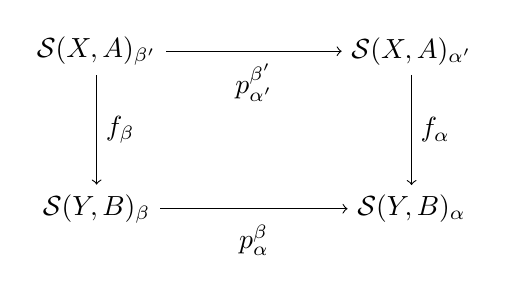
\begin{tikzpicture}
	
	
	
	\node (w) at (0,0) {\(\mathcal{S}(X,A)_{\beta'}\)};
	
	\node (x) at (0,-2) {\(\mathcal{S}(Y,B)_{\beta}\)};
	
	\node (y) at (4,-2) {\(\mathcal{S}(Y,B)_{\alpha}\)};
	
	\node (z) at (4,0) {\(\mathcal{S}(X,A)_{\alpha'}\)};
	
	\node (f) at (2,-2.4){\(p^\beta_\alpha\)};
	
	\node (g) at (2,-0.4){\(p^{\beta'}_{\alpha'}\)};
	
	\node (s) at (0.3,-1) {\(f_{\beta}\)};
	
	\node (s2) at (4.3,-1) {\(f_{\alpha}\)};	
	
	\draw[->] (z) -- (y);
	\draw[->] (w) -- (x);
	\draw[->] (x) -- (y);
	\draw[->] (w) -- (z);
	
	
	\end{tikzpicture}
	$$

\end{lem}

\begin{proof}
Let $\{U_i\}_{i \in J}$ be some simplex in $\mathcal{S}(X,A)_{\beta'}$. For every edge $U$ the set $f^{-1} \circ p \circ f(U) $ is non-empty because $p$ maps $f(U)$ to a larger set. Thus for every edge $U_i$ there is a corresponding edge in $\mathcal{S}(X,A)_{\alpha'}$. We can now define a map $p^{\beta'}_{\alpha'}: \mathcal{S}(X,A)_{\beta'} \rightarrow \mathcal{S}(X,A)_{\alpha}$ in such way that the edge $U$ is mapped to the edge $f^{-1}pfU $ and we extend this map by linearity. Now, by defining the map $p^{\beta'}_{\alpha'}$ in such way for every simplex, we get a well-defined map that makes the diagram commute.
\end{proof}

\chapter{Cech homology}

In this chapter we will construct Cech homology and prove the main results related to it.  We will first define an inverse system of homology groups of the nerves.

\begin{maar}
Let $\alpha$ be an element of $\text{COV}(X,A)$ and let $G$ be an abelian group. Then we can define the group $H_{q,a}(X,A;G)$ using the singular homology groups in the following way: 
$$H_{q,a}(X,A;G) = H_q(\mathcal{S}(X,A)_{\alpha};G).$$ 
For all coverings of $\alpha, \beta$ in $(X,A)$ with $\alpha \leq \beta$ we define the maps to be
$$I^{\beta}_{\alpha}: H_{q,\beta} \rightarrow  H_{q,\alpha}$$ 
maps $I_{\beta}^{\alpha}$ are induced by some maps $p^\beta_\alpha$ which are unique up to homotopy.
\end{maar}
\begin{lem}
Let $q \in \N$ be s fixed number. Let $(X,A)$ be a topological pair and let $G$ be abelian group. Then the groups $H_{q,a}(X,A;G)$ together with maps $I_{\beta}^{\alpha}$ form an inverse system of groups.
\end{lem}
\begin{proof}
First we have to show that $I_{\alpha}^{\alpha}$ is identity function for every $\alpha \in$ COV$(X,A)$. We already know that identity map between simplicial complexes is projection map and because identity map induces identity map between the complexes by uniqueness of $I_{\alpha}^{\alpha}$ we see that the map has to be identity map between corresponding homology groups.\newline Now for every coverings $\alpha, \beta, \gamma$ of pair $(X,A)$ for which relation $\alpha \leq \beta \leq \gamma$ holds we have to show that $I_{\beta}^{\gamma} \circ I_{\alpha}^{\beta} = I^{\gamma}_{\alpha}$. By lemma \ref{compofprojmaps} the composition of corresponding projection maps $p_{\beta}^{\gamma} \circ p_{\alpha}^{\beta}$ is projection map. Thus it defines map $I^{\gamma}_{\alpha}$.
\end{proof}
Now we are ready to define the cech homology groups $ \check{\mathrm{H}}_n$.
\begin{maar}
Let $(X,A)$ be topological pair and $G$ abelian group. Then cech homology groups with coefficients $G$ are defined to be inverse limits of $H_{q,\alpha}(X,A;G)$ where $\alpha$ belongs to COV$(X,A)$. Simply denoted  $\check{\mathrm{H}}_q(X,A;G) = \lim_{\rightarrow}\{H_{q,\alpha}(X,A;G)\}$

\end{maar}
Because coverings can be infinite the limits are not necessary defined. However there is a way to evade this problem. 

\section{Well-definedness of the Cech homology groups}
In this section we will provide condition for the spaces which will guarantee that the Cech groups are well-defined. 
...
From now on in this chapter we assume that the topological spaces are such for which the Cech groups  are well-defined. 

\section{Induced homomorphisms}
In this section we will investigate properties of induced homomorphism. Earlier we defined Cech homology groups to be limit of the groups induced by coverings of the pair. In section \ref{limitmorphism} we defined concept of limit homomorphism. In next theorem we will show that such homomorphism exists.

\begin{lause}
Let $f:(X,A) \rightarrow (Y,B)$ be continuous function between pairs of spaces. Let $\mathcal{A} = \{f_\alpha \mid \alpha \text{ is covering of pair }(Y,B)\}$ be family of functions for which every element of the open covering $\alpha$ is mapped to its preimage. This family induces maps between corresponding cech homology groups. $$f'_{\alpha,q}:H_q(\mathcal{S}(X,A)_{f^{-1}\alpha}; G) \rightarrow H_q(\mathcal{S}(Y,B)_{\alpha}; G)$$
We denote a family of functions indexed by coverings of $(Y,B)$ described above with $\mathcal{A}_q$. Then every such collections is natural transformation of the Cech homology groups and the limit function is well defined. 
\end{lause}
\begin{proof}
We can define a functor $\phi:\text{COV}(Y,B) \rightarrow \text{COV}(A,B)$ to map every object $\alpha$ to $f^{-1}\alpha$. By lemma \ref{preimageorder} this functor preserves order. Let $\beta$ and $\alpha$ be some coverings of pair $(Y,B)$. We denote $\alpha'$ and $\beta'$ to be the preimage categories of $\alpha$ and $\beta$ under map $f$. The diagram of lemma \ref{squarelemmaforcoverings} shows that the corresponding maps between coverings commute. Thus we have a following commutable diagram:
	$$
	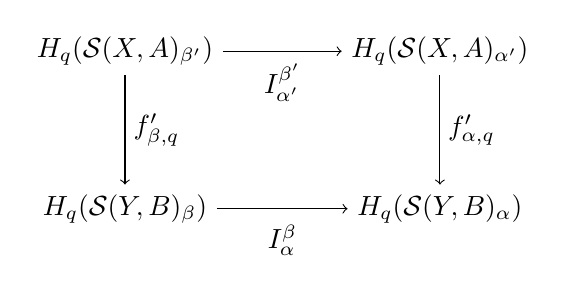
\begin{tikzpicture}
	
	
	
	\node (w) at (0,0) {\(H_q(\mathcal{S}(X,A)_{\beta'})\)};
	
	\node (x) at (0,-2) {\(H_q(\mathcal{S}(Y,B)_{\beta})\)};
	
	\node (y) at (4,-2) {\(H_q(\mathcal{S}(Y,B)_{\alpha})\)};
	
	\node (z) at (4,0) {\(H_q(\mathcal{S}(X,A)_{\alpha'})\)};
	
	\node (f) at (2,-2.4){\(I^\beta_\alpha\)};
	
	\node (g) at (2,-0.4){\(I^{\beta'}_{\alpha'}\)};
	
	\node (s) at (0.4,-1) {\(f'_{\beta,q}\)};
	
	\node (s2) at (4.4,-1) {\(f'_{\alpha,q}\)};	
	
	\draw[->] (z) -- (y);
	\draw[->] (w) -- (x);
	\draw[->] (x) -- (y);
	\draw[->] (w) -- (z);
	
	
	\end{tikzpicture}
	$$
	
The fact that collection $\mathcal{A}_q$ is natural transformation of the groups follows directly from the above diagram. Thus by lemma \ref{limitmorphismgroup} there exists limit homomorphism $$f_q:\check{\mathrm{H}}_q(X,A;G) \rightarrow \check{\mathrm{H}}_q(Y,B;G) $$
\end{proof}
We will show now that the Cech homology group is a functor. 
\begin{lause}
Cech homology groups are functors from the category of the topological pairs to the category of abelian groups 
\end{lause}
\begin{proof}
\begin{enumerate}[label=(\arabic*),ref=(\arabic*)]
\item Every pair of spaces is mapped uniquely to some abelian group.
\item The limit of identity map is an identity homomorphism.
\item Let $f:(X,A) \rightarrow (Y,B)$ and $g:(Y,B) \rightarrow (Z,C)$ be continuous maps between pairs. We know that $(g \circ f)_{*} = g_* \circ f_*$ holds for the singular homology groups. Then by using theorem \ref{compositionlimitmorphism} we see that the limit homomorphism $\lim ((g \circ f)_*)$ equals $\lim g_* \circ \lim f_*$.
\end{enumerate}
\end{proof}


\section{Dimension axiom}
In this section we will prove that the cech homology theory satisfies the dimension axiom.
\begin{lause}
Let $X = \{x\}$ be a space which consist of one point. Then the cech homology groups $\check{\mathrm{H}}_n(X; G) $ are trivial groups for $n \geq 1$ and isomorphic to $G$ when $n = 0$.
\end{lause}
\begin{proof}
For the space $X$ there exists only one open covering $\alpha = \{x\}$ and thus the inverse system of the corresponding singular homology groups is trivial. It is easy to see that the limit of this system is the group $H_q(\mathcal{S}(X)_a; G)$ together with the identity homomorphisms. The simplex $\mathcal{S}(X)_{\alpha}$ consists only of one edge and thus is homeomorphic to a one point space. From the dimension axiom of singular homology it is easy to see that
$$\check{\mathrm{H}}_n(X; G) = \left\{
	\begin{array}{ll}
		G  & \mbox{if } n = 0 \\
		0 & \mbox{if } n \geq 1
	\end{array}
\right. $$
\end{proof}

\section{Homotopy axiom}
The main result of this section is the homotopy axiom of Cech homology which states that if two spaces are homotopic then their all Cech homology groups are isomorphic. In the beginning we will prove an important result regarding the singular homology groups of the nerve of the unit interval $[0,1]$. 

\begin{maar}
Let $X$ be a topological space and $\alpha$ its finite open covering. Then $\text{CLEAN}(\alpha)$ is a covering of space $X$, which is formed by removing every such element $A \in \alpha$ for which $A \subset B$ holds for some $B \in \alpha$ from the collection.
\end{maar}

\begin{lem}\label{cleanlemma}
Let $X$ be a topological space and $\alpha$ its finite open covering. Let $\beta = \text{CLEAN}(\alpha)$ be the covering defined in previous definition. Then singular homology $H_q(\mathcal{S}(X)_{\alpha})$ and $H_q(\mathcal{S}(X)_{\beta}) $ are isomorphic for every $q \in \N$.
\end{lem}
\begin{proof}
Because $\beta$ is subcollection of $\alpha$, the relation $\alpha \leq \beta$ holds. Relation $\beta \leq \alpha$ holds, because if we take any element from $a \in \alpha$ which is not in $\beta$ by definition we will find an element $b \in \beta$ for which the relation $a \subset b$ holds. \newline
Thus there exists morphisms $I^{\beta}_{\alpha}$ and $I^{\alpha}_{\beta}$ in the inverse system of abelian groups induced by coverings. By definition equations $I^{\beta}_{\alpha} \circ I^{\alpha}_{\beta} = I^{\beta}_{\beta} = id_{\beta}$ and $I^{\alpha}_{\beta} \circ I^{\beta}_{\alpha} = I^{\alpha}_{\beta} = id_{\alpha}$ hold. Thus $I^{\beta}_{\alpha}$ is an isomorphism between $H_q(\mathcal{S}(X)_{\alpha})$ and $H_q(\mathcal{S}(X)_{\beta}) $. 
\end{proof}
\begin{maar}
	Let $\alpha$ be a cleaned finite open covering of $[0,1]$, for which every element in the collection is connected. Trivial indexation of $\alpha$ is the following indexation: We order open intervals in the collection $(a,b) \in \alpha$ by the cordinate $a$ and number coverings.
\end{maar}
\begin{lem}
Let $\alpha$ be a open covering of $[0,1]$m which is cleaned, finite and connected. Then the trivial indexation $[m]$ preserves order of the coordinate $b$ of open intervals.
\end{lem}
\begin{proof}
If $b_n > b_{n+1}$ for some $n \in [m-1]$, then $(a_{n+1},b_{n+1}) \subset (a_{n}, b_n)$ which is a contradiction by the definition of the covering $\alpha$.
\end{proof}

\begin{lem}
Let $\alpha$ be an open covering which is finite and every element in the collection is connected. Then every singular homology group of the nerve $\mathcal{S}([0,1])_{\alpha}$ is trivial. 
\end{lem}
\begin{proof}
Using \ref{cleanlemma} we can reduce our problem to coverings which have property that no inclusion holds for any two element of the collection $\alpha$. We define indexation to be trivial indexation for covering $\alpha$. Let $\{f_n(x):\mathcal{S}([0,1])_{\alpha} \rightarrow  \mathcal{S}([0,1])_{\alpha} \}_{n \in [m]}$ be a collection of simplicial maps which are induced by the edges in the following way:
$$f_n(v_i) = \left\{
\begin{array}{ll}
v_i  & \mbox{if } i \leq n \\
v_n & \mbox{if } i \geq n
\end{array}
\right.$$
We will now show that the maps defined above induce same homomorphisms between the corresponding groups. Because the indexation set is finite, it is enough to show that $f_{n}$ and $f_{n+1}$ are contiguous for every $n$ in the collection. Let $s$ be some simplex in the nerve $\mathcal{S}([0,1])_{\alpha}$. If simplex $s$ is spanned only by elements whose index is less than $n$, maps $f_{n}$ and $f_{n+1}$ are both identity on it. Now assume that $s$ contains atleast one edge the index of which is larger than $n-1$. Then the image of the element $s$ under the map $f_{n}$ can be presented as $\rhd(s',v_n)$, where $s'$ is simplex for which index of every edge is smaller than $n$. There are two possible representations for the image $f_{n+1}(s)$ namely $\rhd(s',v_n,v_{n+1})$ and $\rhd(s\,v_{n+1})$. If the representation of $f_{n+1}(s)$ is $\rhd(s',v_n,v_{n+1})$, we can choose the simplex to be $\rhd(s',v_n,v_{n+1})$, as it clear from definition that $\rhd(s',v_{n+1})$ is its face. In the second case we notice that because intersection $\bigcap_{a \in s'}a \cap v_{n+1}$ is non-empty and connected. Thus it is an open interval $(a_{n+1},b_{1}) $. Because condition $(a_n,b_n) \cap (a_{n+1},b_{1}) \neq \emptyset$ holds, we can choose $\rhd(s',v_n,v_{n+1})$ to be the simplex where image of $s$ of the both functions are contained.
\end{proof}
Next we define a class of nice coverings for the unit interval $[0,1]$ and prove that the subcategory which consists of the coverings defined is a subcategory of the Cech inverse system. 

\begin{maar}
Let $\alpha = \{U_i\}_{i \in [n]}$ be a connected open covering of unit interval $[0,1]$ for which the following conditions are satisfied:
\begin{enumerate}[label=(\arabic*),ref=(\arabic*)]
	\item $0 \in U_0$ and $1 \in U_n$
	\item $U_i \cap U_{i+1} \neq \emptyset$ for every $i \in [n-1]$ 
	\item $U_i \cap U_j = \emptyset$ for all $|i - j| \geq 1$
\end{enumerate}
Then we say that covering $\alpha$ is regular.
\end{maar}
\begin{lem}
The category of the regular coverings of $[0,1]$ is cofinal in the $COV([0,1])$.
\end{lem}
\begin{proof}
Let $\alpha$ be arbitrary covering of $[0,1]$. We modify the covering in the following ways:
\begin{enumerate}[label=(\arabic*),ref=(\arabic*)]
\item  We form covering $\beta$ by selecting some finite subcovering of $\alpha$. 
\item  We split every non-connected element in the collection $\beta$ into connected elements.
\item  We search for the removable elements i.e the the collection after removing the element covers the space $[0,1]$. We remove every such element and stop this process after no removable elements are found.
\item We define the indexation to be the trivial indexation.
\end{enumerate}
The condition (1) and (2) are satisfied , because $\gamma$ is trivially indexed covering. Condition (3) is satisfied, because if two open intervals with are not neighbors have non-empty intersection then all the coverings between can be removed and that collection will still cover the set. Because covering $\gamma$ is obtained by removing and cutting elements, the relation $\beta \leq \gamma$ holds.
\end{proof}
\begin{maar}
Let $(X,A)$ be topological pair and $\alpha = \{(V_i,U_i)\}_{i \in J}$ its covering. Suppose that for every $V_x$ there is a regular covering $\beta(x)$ of an unit interval $[0,1]$ indexed by the set $[n]$ for some $n \in \N$. Covering $\gamma$ of the pair $(X \times [0,1], A \times [0,1]) $ defined in the following way:
$$\gamma = \{(V_x \times \beta(x), V_x \times \beta(x))\}_{x \in J} $$
is called a stacked covering over $\alpha$.
\end{maar}
\begin{lem}
The category of stacked coverings is cofinal in $COV((X \times [0,1], A \times [0,1]))$
\end{lem}
\begin{proof}
Let $\gamma = {(V_i, U_i)}_{i \in J}$
\end{proof}

\chapter{Applications}

\section{Lefschetz fixed-point theorem}
[Theory of this will be presented later]

\section{Kakutani fixed point theorem}

The fixed point theorem of Kakutani can be derived for Lefchetz fixed-point theorem.

\begin{maar}
Let $X$ be vector space with topological structure and $K$ topological field. If vector addition $+:X \times X \rightarrow X$ and scalar multiplication $\cdot:K \times X \rightarrow X $ are continuous we say that $X$ is topological vector space over field $K$ or shortly $L(X,K)$ 
\end{maar}
Topological vector space has following property:
\begin{lause}
Kakutani fixed point theorem. Let $S$ be a non empty, compact and convex subset of a locally convex Hausdorff space. Let $f:S \rightarrow 2^s$ be a multivalued function on $S$ which has closed graph and the property that $f(x)$ is convex and non-empty for all $x \in S$. Then the set of fixed points of $f$ is non-empty and compact.
\end{lause}



\section{Continuous game theory}
In this section we will apply theory developed in previous chapters to game theory. We define $n$ player continuous game structure $Cgs(J, \mathcal{A})$ in a following way:

\begin{maar}
Let $J$ be finite indexing set and $\mathcal{A}$ collection of continuous utility functions $\{u_i:X_i \rightarrow \R \}_{i \in J}$ with a compact domain. Then we say that $Cgs(J, \mathcal{A})$ is a continuous game.
\end{maar}
Now we give definition of Nash equilibrium for Cgs.

\begin{maar}
Let $Cgs(J, \mathcal{A})$ be continuous game we say that point $x^{*} \in \prod_{i \in J}X_i$ is Nash equilibrium if for every $k \in J$ and every $x'_k \in X_k$ following condition holds:
$$u_k(x*) \geq u_k(x_1, ..., x'_k, ... , x_n) $$ 
\end{maar}
Next we will prove important lemma which says that game has equilibrium only and only if specific function has fixed point. 
\begin{lem}
$Cgs(n, \mathcal{A})$ has Nash equilibrium only and only if following set value function $$g:\prod_{i \in J}X_i \rightarrow \prod_{i \in J}2^{X_i}: g_k(x) = \argmax_{t \in X_k}u_k(x_1, ... x_{k}, t, x_{k+1},...,x_{n})$$
has a fixed point $x \in g(x)$  
\end{lem}
\begin{proof}
Trivial (Just check definitions)
\end{proof}

\subsection{General version of resource optimization problem}
Consider a game where a set of players compete in a multiple competitions at the same. Every player has limited energy and they can allocate it freely. Every competition is won by a player who allocated most energy in it and the goal of the players is to maximize the amount of the competitions they win.

\begin{maar}
We define the continuous game structure of the game described above as follows:
\begin{enumerate}
\item The choice space for every player consists of continuous functions $f:[0,1]\rightarrow \R$ for which $\int_{0}^{1}f(x) dx = 1 $
\item The evaluation function $u_n(x):\prod_{i \in J}X_i \rightarrow [0,1]$ is defined to be: $$u_n(f) = m^*(\{x \in [0,1] \mid f_n(x) \geq f_i(x)\})$$
\end{enumerate}
\end{maar}
We will show that in some cases there exists an equalibrium.


\begin{appendices}

\chapter{Homology axioms}
For homology theories we have a following interface:
\begin{maar}
A homology theory consists of a family of the functors from category of topological pairs to category of abelian groups $\{H_n\}_{n \in \N}$ and natural transformations $\{\delta_n:H_n(X,A) \rightarrow H_{n-1}(A,\emptyset)\}_{n \in \N} $ . For the homological theory the following axioms are satisfied:
\begin{enumerate}
\item text here
\end{enumerate} 
\end{maar}

\end{appendices}


\begin{thebibliography}{9}

\bibitem{Rotman}\label{rotman}

J. Rotman An Introduction to Algebraic Topology (Graduate Texts in Mathematics), Springer 

\bibitem{First}
L. G�rniewicz, Topological Fixed Point Theory of Multivalued Mappings, Kluwer Academic
Publishers, 1999.

\bibitem{Second} 
I. L. Glicksberg, A further generalization of the Kakutani fixed point theorem with
application to Nash equilibrium points, Proc. Amer. Math. Soc. 3 (1952), 170�174.


\bibitem{Vaisala}\label{vai}
M. BAYE, G. TIAN, ANU J. ZHOU, �The Existence of Pure Nash Equilibrium in Games 
with Nonquasiconcave Payoffs,� Texas A  M University, mimeo, 1990. 

\bibitem{categorytheory}\label{categorytheory}
Saunders Mac Lane: Categories for the Working Mathematician (Graduate Texts in Mathematics)

\bibitem{algebra2}\label{algebra2}
Jokke H�s�: Algebra II, 2016. 

\end{thebibliography}

\end{document}
